\chapter{Visualisation Evaluation}\label{C:sd}
Following the completion of the implementation stage of this project a final
user evaluation was carried out on the visualisation. This evaluation was
primarily designed to discover whether or not the visualisation created was
successful in fulfilling the requirements of the project.

\section{Why was evaluation conducted}
Visualisation methods are often designed and evaluated by presenting 
results informally to potential users. No matter how 
efficient a visualisation technique may be, or well planeed it is, if it does
not convey information 
effectively, it is of little use. User studies offer a 
scientifically sound method to measure a visualisation’s 
performance. There are many reasons to pursue user studies. Studies can 
be used to evaluate the strengths and weaknesses of 
different visualization techniques or show that a visualization technique is 
useful in a practical sense, according to some objective 
criteria, for some specific task \cite{kosara2003thoughts}. 

A more fundamental goal of conducting user studies is to 
seek insight into why a particular technique is effective. 
This can guide future efforts to improve existing 
techniques. We want to understand for what types of tasks, 
and under what conditions, a particular method will give 
high quality results \cite{kosara2003thoughts}.

The evaluation of this project was designed to qualitatively assess users
reactions and experiences with the IKVT. By mapping users experiences to the
project
requirements I was able qualitatively evaluate how successful the visualisation
was a fulfilling these requirements.

~Why not quantitative
 - statistically significant. 
\section{User Study Method}
A poorly designed experiment will only yield results of limited value, because
of this it was important to ensure that each stage of the experiment was
focussed on evaluating a specific area of the viusalisation in relation to the
project requirements.

There were 3 key methods of gathering results during this evaluation; a
worksheet to fill out whilst using the visualisation made up of 2 sets of questions(one for the keyboard \& mouse system and one for the Kinect system)(APPENDIX), a questionnaire to
fill in afterwards about the experience (APPENDIX), and the examiners observations about
how the users interacted with the system.  
\\\\
The following are the steps that were carried out during each user evalutation to ensure that the variables were the same each time
\begin{itemize}
\item The user enters the room and sits down at the computer.
\item They are handed the consent form and information sheet.
\item After these are completed they are handed the user questionnaire and the
set of questions to answer while using the system. On this questionnaire there
are two sets of questions, the first is for the keyboard and mouse system, and
the second if for the Microsoft Kinect system.
\item Following this they are advised that they have 5 minutes to get
familiarised with the system but they do not need to use all of this time (the
amount of time taken will be recorded for analysis of how user friendly and
intuitive the system is).
\item Following this the user is asked to complete the worksheet by first
using the mouse and keyboard system. When they feel they have answered the first set of questions they will notify the examiner who will move the user to the Kinect
system to continue with the second set.
\item Once the user has completed both sets of questions they are asked to fill
in the qualitative user questionnaire about their experiences using the
visualisation. 
\item Following this if the examiner has no follow up questions the user is free
to leave.
\end{itemize}

\section{Evaluation Environment}
\begin{figure}[H]
  \centering
      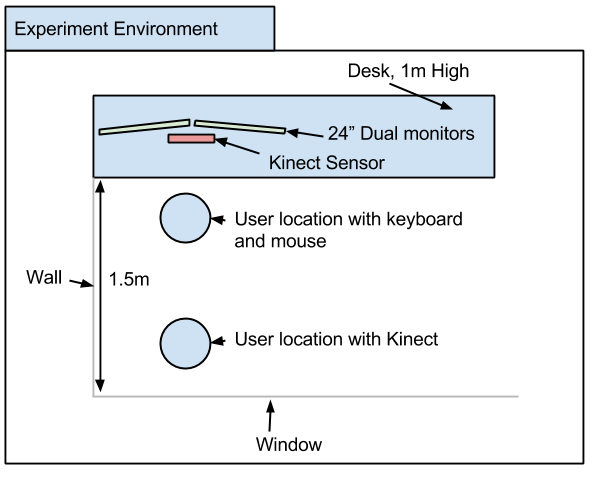
\includegraphics[width=0.8\textwidth]{images/environment.png}
  \caption{Evaluation environment}  
    \label{fig:environment}
\end{figure}

\section{Expectations of evaluation}
From this evaluation the expectations were that users would take approximately 3
minutes to feel comfortable with using the visualisation for the basic tasks of
moving the camera around, sorting the exoplanets, and using the range sliders to
filter the exoplanets. 

Following this accostomisation time it was expected that users could accurately
complete the set of questions in a worksheet (APPENDIX QUESTIONS) whilst using
the visualisation. During this stage users are expected to use both interaction
methods (Keyboard \& Mouse, and Kinect sensor). During the keyboard \& mouse
portion of the experiment the users should make more accurate selections and
exhibit more effective data seeking behavior, whereas during the Kinect portion
they would be more interesting in experimenting with gestures rather than
attempting to gain information about exoplanets. 

When users have finished using the visualisation and fill in the questionnaire
asking them about their experiences with the system the expectation was that
they would detail the areas of the visualisation that ...~


\subsection{Participants}
The user study was undertaken by 9 participants P2 to P10 as well as a 1 user pilot study by P1, all were either students or
young professionals from a mix of specialties aged between 21 to 26 with a mix
of genders with 5 females and 4 males. 5 of these participants had extensive prior experience with Kinect sensors, and all participants had experienced a 3D visualisation before.

\section{Pilot Study}
Due to the significant costs associated with running an experiment, it 
is valuable to conduct a pilot study with one or two 
participants. This allows testing and refining the experimental
design before starting a full-fledged study with numerous 
participants \cite{kosara2003thoughts}. 

The reason for conducting this pilot study for this project was to ensure that the experiment was
producing the data required to evaluate the the visualisation produced as well
as taking the correct amount of time to complete. In addition to this it was
used to discover whether there were any aspects of the study that would
interfere with the results.

One participant was asked to take part in a pilot study before any results were
collected, this participant is refered to as P1. This participant was asked to complete all of the activities that
make up the main experiment. This pilot study took approximately 15 minutes as
intended, this included the time needed for the explanation and completion of
paperwork, as well as the experiment itself.

P1 successfully each of the questions whilst using the visualisation with only limited assistance from the examiner. This assistance was required due to the wording of
some of the tasks users were asked to complete being ambiguous which caused
unnecessary confusion which could have interfered with the results. These ambiguous questions and
tasks were removed prior to the main user study. During the main study only P4 and P10 asked for clarification on the questions or tasks.

P1 had some initial difficulty using the range sliders but after a small period of experimentation began using them for the majority of tasks which turned out to be very efficient. P1 also found that whist the range sliders were effective, they did not allow fine enough control for making small changes.

The component of the visualisation that P1 had the most difficulty was using the view depticting the location of planets in relation to their stars habitable zones. This difficulty seemed to stem from the lack of a common point of reference for each planet due to each planet having a different star with its own habitable zone.

During the Kinect portion of the experiment P1 found that being in a sitting position whist interacting with the visualisation did not feel natural due to ``being required to reach out and exert effort to hold an upright position of the arms for an extended period of time''. The following figure displays P1s reactions to questions about the experience of using the IKVT.
\begin{figure}[H]
  \centering
      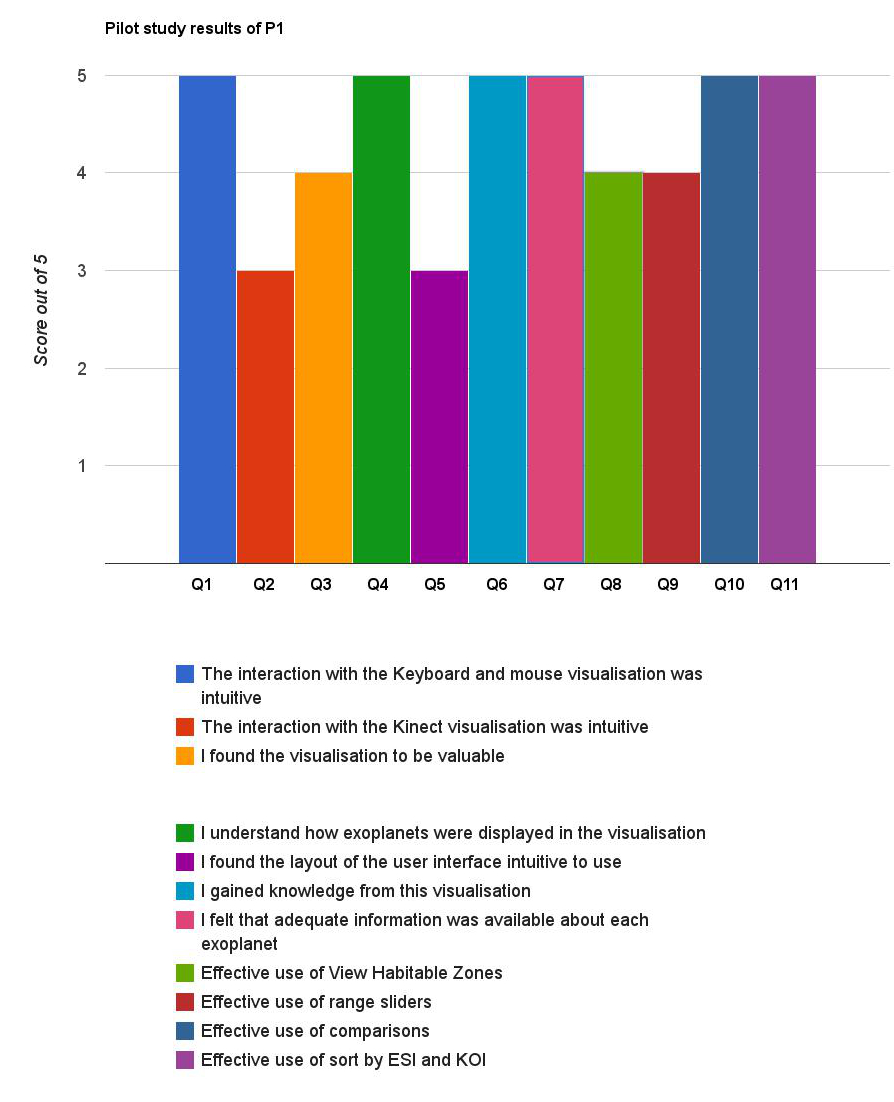
\includegraphics[width=1\textwidth]{images/pilot.jpg}
  \caption{Pilot study results of P1}  
    \label{fig:pilot}
\end{figure}



\section{Evaluation of Keyboard and mouse visualisation}
The keyboard \& mouse portion of the experiment was primarily intended to
evaluate how the interaction techniques that were introduced into the
visualisation can aid users in their information seeking behaviours.
This was evaluated through the first part of the question set that users filled
in whilst using the visualisation. These questions were designed in a way that
encouraged users to make use of each of the interactive features that were
introduced.

\begin{enumerate}
 \item[P2.] 
 P2 found that the information displayed in the IKVT was easy to follow even without knowing exactly what each peice of information actually meant.
 
 P2 also found that without more of an in depth introduction into each of the tools 
  \item[P3.]
   \item[P4.]
    \item[P5.]
     \item[P6.]
      \item[P7.]
       \item[P8.]
        \item[P9.]
         \item[P10.]
\end{enumerate}

\section{Evaluation of Microsoft Kinect visualisation}
The Microsoft Kinect portion of the experiment was intended to evaluate how
users would react to intereacting with the visualisation by gesture. The
questions for this portion of the evaluation were desiged to find out users
experiences with interacting via Kinect.

\begin{enumerate}
 \item[P2.]
  \item[P3.]
   \item[P4.]
    \item[P5.]
     \item[P6.]
      \item[P7.]
       \item[P8.]
        \item[P9.]
         \item[P10.]
\end{enumerate}

\section{Performance evaluation}

\section{Results}
\subsection{Evaluation of Requirements}
\subsubsection{Evaluation of Functional Requirements}
\begin{enumerate}

 \item[R1.] The visualisation needs to display planetary information to convey
knowledge to users.

 \item[R2.] The visualisation needs to allow exoplanets to be compared against
one another.

 \item[R3.] The planets need to be able to be ordered by their similarity to
earth (ESI) and by their Kepler Object of Interest number (KOI).
 
 \item[R4.] The visualisation needs to allow users to define ranges of planetary
attributes to filter which planets are displayed.

 \item[R5.] Users need to be able to view the habitable zones of stars in
relation to the planets orbiting them.

\end{enumerate}

\subsubsection{Evaluation of Nonfunctional Requirements}
\begin{enumerate}
 \item[R6.] All interaction methods must be visible and intuitive.

 \item[R7.] The visualisation must remain uncluttered to reduce information
overload.

 \item[R8.]  There needs to be two modes of interaction with the system,
keyboard and mouse vs gesture based.
\end{enumerate}

\begin{figure}[H]
  \centering
      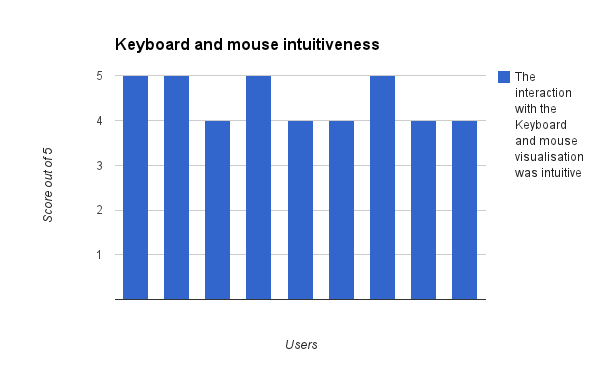
\includegraphics[width=0.8\textwidth]{images/charts/chart_1.png}
  \caption{Intuitivity of keyboard and mouse}  
    \label{fig:chart1}
      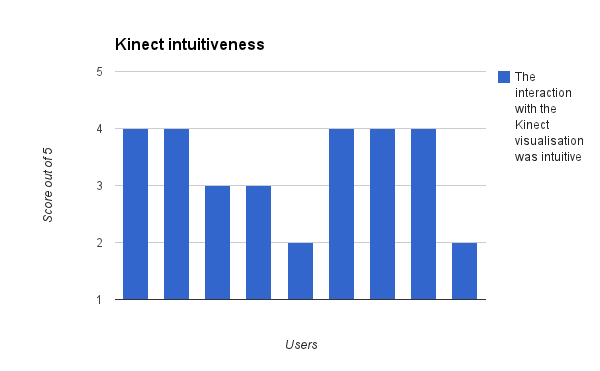
\includegraphics[width=0.8\textwidth]{images/charts/chart_2.png}
  \caption{Intuitivity Microsoft Kinect sensor}  
    \label{fig:chart2}
      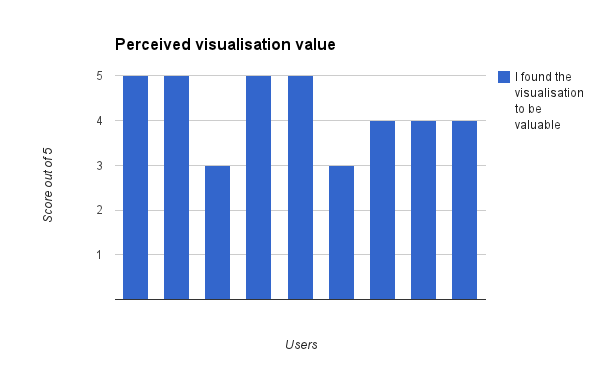
\includegraphics[width=0.8\textwidth]{images/charts/chart_3.png}
  \caption{Perceived value of visualisation}  
    \label{fig:chart3}
\end{figure}

\begin{figure}[H]
  \centering
      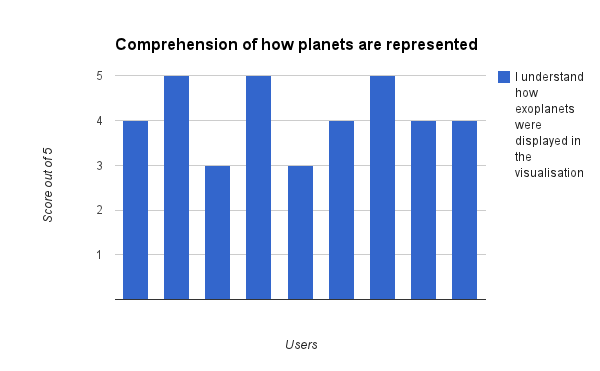
\includegraphics[width=0.8\textwidth]{images/charts/chart_4.png}
  \caption{User comprehension of visualisation}  
    \label{fig:chart4}
      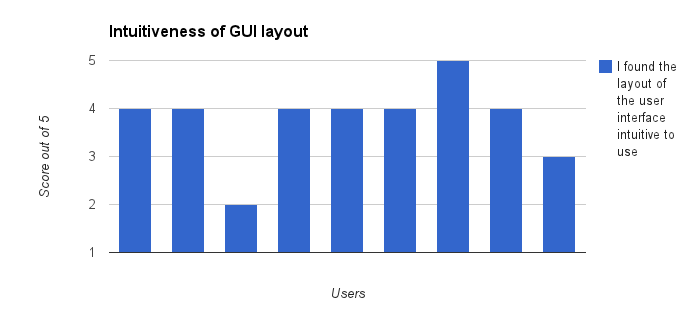
\includegraphics[width=0.8\textwidth]{images/charts/chart_5.png}
  \caption{GUI layout intuitivity}  
    \label{fig:chart5}
\end{figure}

\begin{figure}[H]
  \centering
      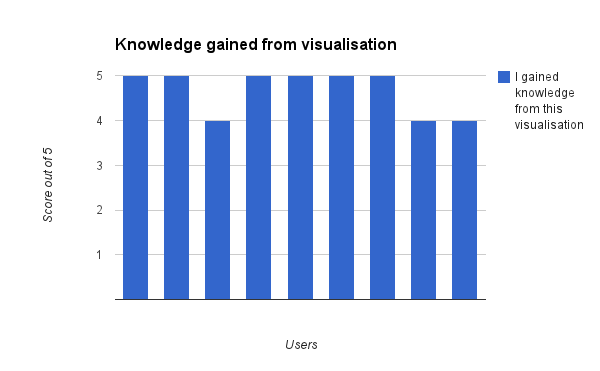
\includegraphics[width=0.8\textwidth]{images/charts/chart_7.png}
  \caption{Knowledge gained from the visualisation}  
    \label{fig:chart7}

      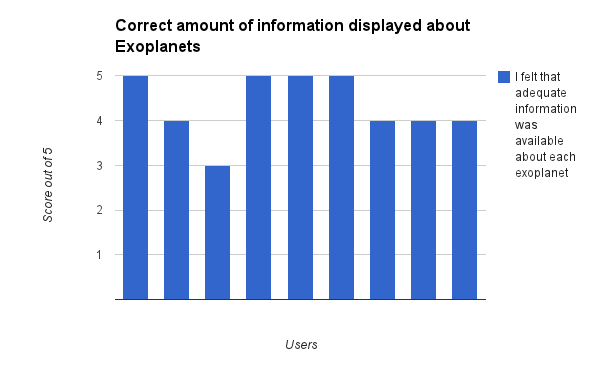
\includegraphics[width=0.8\textwidth]{images/charts/chart_8.png}
  \caption{Correct amount of information displayed}  
    \label{fig:chart8}
      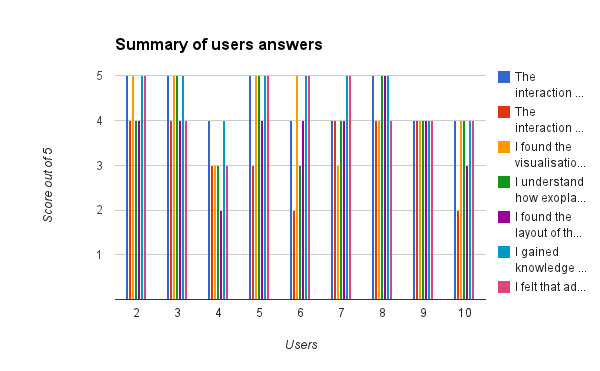
\includegraphics[width=0.8\textwidth]{images/charts/chart_9.png}
  \caption{Summary of results}  
    \label{fig:chart9}
    
\end{figure}
\section{Threats to validity}
Lack of control system

%Are all participants sufficiently willing and able to perform 
%the task? Is there a learning effect? 
%These problems can be addressed by testing participants for 
%adequate spatial acuity, stereo ability, and absence of color 
%blindness, by randomizing the presentation order of the 
%trials, by using written instructions, by allowing 
%participants to rest during the experiment to avoid 
%becoming fatigued, by devising robust methods to identify 
%when participants are giving “garbage answers”, and by 
%asking participants to successfully complete a training task 
%before proceeding to the recorded trials